\section{Gradientenfelder und Potentiale}
\begin{LA}{Einführung}{ArbeitOszillator2D}
    Betrachten wir einen Massenpunkt, der im Ursprung unseres Koordinatensystems so gelagert ist, dass seine Auslenkung in Richtung der Koordinatenachsen, etwa durch zwei Federn realisiert, eine Rückstellkraft proportional zur Auslenkung erfährt, die in  \(y\)-Richtung doppelt so gross sei, wie in \(x\)-Richtung.
    \begin{center}
        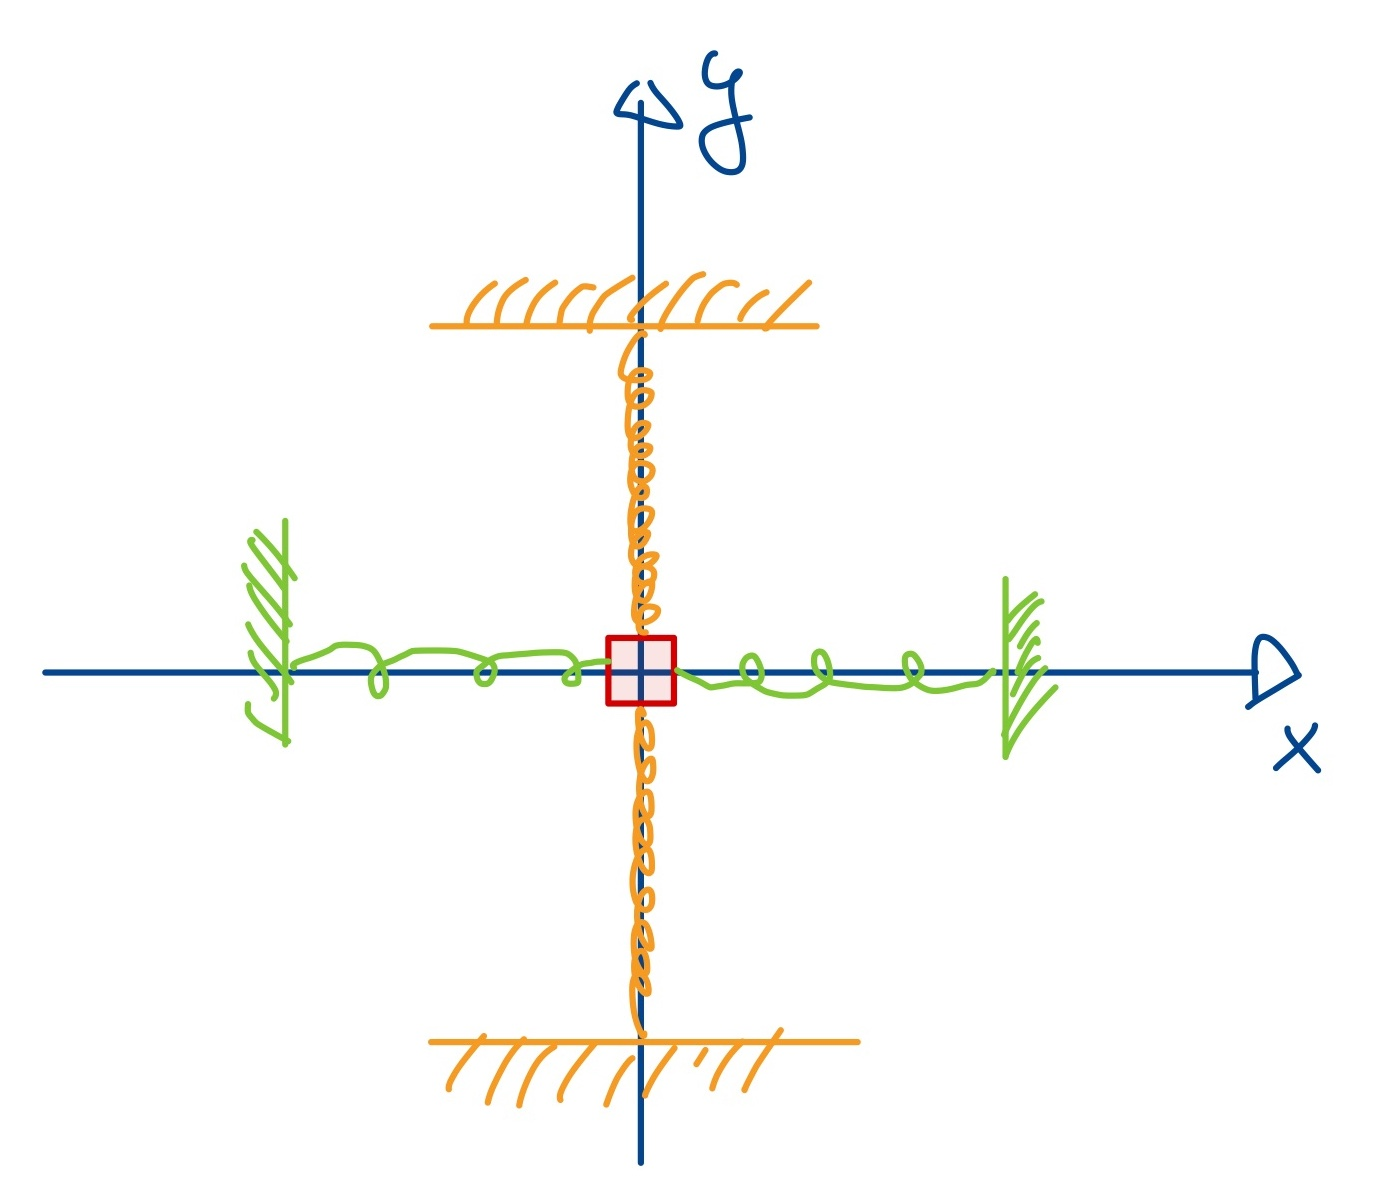
\includegraphics[width=0.5\textwidth]{harmosz2d.jpg}
    \end{center}
    Das wirkende Kraftfeld ist dann \(\vec{F}(x,y)=\begin{pmatrix}
        -x \\ -2y
    \end{pmatrix}\).

    Der Massenpunkt soll nun von der Ruhelage zum Punkt \((-2, 0)\) bewegt werden. Einmal entlang der geraden Verbindung \(\vec{r}_1 : [0,2] \to \R^2, t \mapsto \begin{pmatrix}
        -t \\ 0
    \end{pmatrix}\) und einmal entlang des Halbkreises \(\vec{r}_2 : [0,\pi] \to \R^2, t \mapsto \begin{pmatrix}
        \cos(t) - 1 \\ \sin(t)
    \end{pmatrix}\)

    Berechnen Sie für jeden Weg die verrichtete Arbeit und vergleichen Sie die Resultate.
    (Zur Vereinfachung des Integranden beim Halbkreisweg kann die Doppelwinkelformel helfen: \(\sin(2x) = 2 \sin(x)\cos(x)\) woraus folgt: \(\sin(x)\cos(x)) = \frac{1}{2} \sin(2x)\)


\end{LA}
\clearpage
Im Einführungsbeispiel wird für beide Wege von \((0,0)\) zum Punkt \((-2,0)\) die gleiche Arbeit verrichtet. Das ist kein Zufall!

\begin{satz}
    {Wegunabhängigkeit eines Arbeitsintegrals}{}
    Sei \(\vec{F}: \R^2 \to \R^2\) ein (stetiges) Vektorfeld. Falls es eine Funktion \(\Phi : \R^2 \to \R\) gibt, mit der Eigenschaft \(\vec{\nabla} \Phi = \vec{F}\), dann ist der Wert eines Arbeitsintegrals entlang einer Kurve \(K\) nur von deren Anfangspunkt \(A\) und dem Endpunkt \(B\) abhängig.
    Genauer gilt:

    \[ \int_K \vec{F} d\vec{s} = \Phi(B) - \Phi(A)\]
\end{satz}

Diese Aussage ist quasi die höherdimensionale Entsprechung des Hauptsatzes der Differential- und Integralrechnung aus dem Grundlagefach: \(\int_{a}^{b} f(x) dx = F(b) - F(a)\)


\begin{definition}
    {Gradientenfeld, konservatives Vektorfeld, Potential}{}
    Ein Vektorfeld \(\vec{F}\) mit der Eigenschaft \(\vec{\nabla} \Phi = \vec{F}\) nennt man ein Gradientenfeld oder ein konservatives Vektorfeld.

    Die Funktion \(\Phi\) nennt man das zugehörige (Skalar-)Potential.
\end{definition}
\begin{bsp}
    {Potential des zweidimensionalen Oszillators}{
    }
    Betrachten wir noch einmal das Kraftfeld aus \Cref*{LA:ArbeitOszillator2D}: \(\vec{F}(x,y)=\begin{pmatrix}
        -x \\ -2y
    \end{pmatrix}\).

    Man kann leicht einsehen, dass \(\vec{F}\) das Gradientenfeld des Potentials \(\Phi(x,y) = -\frac{1}{2} x^2 - y^2\) ist.

    Für die beiden Wege \(\vec{r}_1\) und \(\vec{r}_2\) aus \Cref*{LA:ArbeitOszillator2D}, welche die beiden Punkte \(A=(0,0)\) und \(B=(-2,0)\) verbinden, gilt dann:
    \[\int_{\vec{r}_1} \vec{F} d\vec{s} =\int_{\vec{r}_2} \vec{F} d\vec{s} = \Phi(-2,0) - \Phi(0,0) = -\frac{1}{2} (-2)^2 = -2\]

\end{bsp}

Das Beispiel gibt auch eine physikalische Interpretation des Potentials. Mit der Funktion \(\Phi\) im Beispiel des zweidimensionalen Oszillators lässt sich die potentielle Energie (im Fall der Feder heisst das Spannenergie) des Massenpunkts berechnen. Es gilt nämlich: Die Spannenergie eines Massenpunktes, der sich an der Stelle \((x,y)\) im Kraftfeld \(\vec{F}\) befindet, ist \(E_{\text{spann}} = - \Phi(x,y)\). Der Wert des Arbeitsintegrals ist dann die Differenz der Spannenergie am Anfangspunkt und jener am Endpunkt des Weges.\footnote{Im Kontext der Physik wird das Potential darum auch häufig als die Funktion definiert, für welche \(\vec{\nabla} \Phi = - \vec{F}\) ist.}

\begin{bsp}
    {Das Wirbelfeld ist kein Gradientenfeld}{AnsatzmethodefürPotential}
    Wir betrachten nochmals die Situation aus \Cref*{bsp:Wirbelfeld2Wege}. Wie wir dort bereits berechnet haben, gilt für das Vektorfeld \(\vec{F}(x,y) = \begin{pmatrix}
        -y \\x
    \end{pmatrix}\) und für die beiden Kurven
    \[\vec{r}_1 : [0,1]\to \R^2, t \mapsto \begin{pmatrix}
            1-2t \\ 0
        \end{pmatrix}  \quad \text{und}\quad  \vec{r}_2 : [0, \pi]\to \R^2, t \mapsto \begin{pmatrix}
            \cos t \\ \sin t
        \end{pmatrix}  \]
    dass
    \[ \int_{\vec{r}_1} \vec{F} \, d\vec{s} = 0 \, \neq \int_{\vec{r}_2} \vec{F} \, d\vec{s} = \pi\]

    Obwohl beide Kurven von \(A=(1,0)\) nach \(B=(-1,0)\) verlaufen, haben die Integrale einen unterschiedlichen Wert. Das liegt darin, dass das Vektorfeld \(\vec{F}\) kein Gradientenfeld ist. Das lässt sich leicht einsehen:

    \vspace*{15cm}

    %    Angenommen es gäbe eine Funktion $\Phi: \R^2 \to \R$ mit $\vec{\nabla}\Phi(x,y) = \vec{F}(x,y) = \begin{pmatrix}
    %     -y \\x
    %    \end{pmatrix}$. Dann müsste 
    %    $$\frac{\partial\Phi(x,y)}{\partial x} = -y$$
    %    sein. Durch Integration nach $x$ folgt:
    %    $$\Phi(x,y) = -xy + c_1 (y)$$
    %    Wobei $c_1(y)$ ein Term ist, der zwar von $y$ nicht aber von $x$ abhängig ist.

    %    Gleichzeitig muss auch
    %    $$\frac{\partial\Phi(x,y)}{\partial y} = x$$
    %    gelten. Woraus wieder durch Integration – diesmal nach $y$ – folgt:
    %    $$\Phi(x,y) = xy + c_2(x)$$
    %    Insgesamt erhält man:
    %    $$-xy + c_1 (y)=\Phi(x,y) = xy + c_2(x) \iff c_1(y)+c_2(x)=2xy$$
    %    Diese Gleichung ist offensichtlich für keine Wahl der Termen $c_1(y)$ und $c_2(x)$ erfüllbar.

\end{bsp}
Für die Berechnung von Arbeitsintegral der Form \(\int_{K} \vec{F} \, d\vec{s}\) empfiehlt sich das folgende Vorgehen:
\begin{itemize}
    \item Versuche dem \Cref*{bsp:AnsatzmethodefürPotential} folgend, ein Potential \(\Phi\) zu finden mit \(\vec{\nabla}\Phi = \vec{F}\)
    \item Wenn erfolgreich: \(\int_{K} \vec{F} \, d\vec{s} = \Phi(B)-\Phi(A)\), wobei \(A\) der Anfangs- und \(B\) der Endpunkt der Kurve ist.
    \item Wenn nicht erfolgreich (oder nicht möglich): Berechne \(\int_{K} \vec{F} \, d\vec{s} =\int_{a}^{b}\langle \vec{F}(\vec{r}(t)), \dot{r}(t) \rangle  \,  dt\)
\end{itemize}

Um zu entschieden, ob ein Vektorfeld ein Gradientenfeld ist, kann man manchmal auch die folgende Überlegung verwenden. Wir erinnern uns, dass für eine zweimal stetig differenzierbare Funktion \(\Phi: \R^2 \to \R\) die gemischten partiellen Ableitungen gleich sind, also
\begin{satz}
    {Satz von Schwarz}{
    }
    Sei \(\Phi: \R^2 \to \R\) eine zweimal stetig differenzierbare Funktion. Dann gilt:
    \[\frac{\partial^2 \Phi}{\partial x \partial y} = \frac{\partial^2 \Phi}{\partial y \partial x}\]
\end{satz}

Für ein Gradientenfeld \(\vec{F} = \begin{pmatrix}
    F_1 \\ F_2
\end{pmatrix} = \vec{\nabla} \Phi = \begin{pmatrix}
    \frac{\partial \Phi}{\partial x} \\ \frac{\partial \Phi}{\partial y}
\end{pmatrix}\) gilt also:
\[  \frac{\partial F_2}{\partial x}-\frac{\partial F_1}{\partial y} =  \frac{\partial^2 \Phi}{\partial x \partial y}-\frac{\partial^2 \Phi}{\partial y \partial x}  = 0\]

\begin{definition}
    {Rotation}{}
    Sei \(\vec{F} = \begin{pmatrix}
        F_1 \\ F_2
    \end{pmatrix}\) ein Vektorfeld. Dann nennt man den Ausdruck
    \[\text{rot}(\vec{F}) = \frac{\partial F_2}{\partial x} - \frac{\partial F_1}{\partial y}\]
    die Rotation von \(\vec{F}\).
\end{definition}

\begin{satz}
    {Notwendige Bedingung für ein Gradientenfeld}{}
    \(F\) ist ein Gradientenfeld \(\implies \text{rot}(\vec{F}) = 0\)

    Oder anders formuliert: \(\text{rot}(\vec{F}) \neq 0 \implies F\) ist kein Gradientenfeld.
\end{satz}
Bemerkung: Unter bestimmten Voraussetzungen (z.B. wenn der Definitionsbereich von \(\vec{F}\) einfach zusammenhängend ist) gilt auch die Umkehrung: \(\text{rot}(\vec{F}) = 0 \implies F\) ist ein Gradientenfeld.
\clearpage
\begin{ueb}
    {}{}

    \begin{enumerate}
        \item Berechnen Sie das Kurvenintegral des Vektorfeldes \(\vec{F}(x,y)=\begin{pmatrix}
                  x^2 \\y^2
              \end{pmatrix}\) entlang der Wege \( \vec c_1 \) und \( \vec c_2 \):

              \[
                  \quad \vec c_1 : [0,1] \rightarrow \mathbb{R}^2, \quad \vec c_1(t) = \begin{pmatrix} t \\ t \end{pmatrix} \quad \text{bzw.} \quad \vec c_2 : [0,1] \rightarrow \mathbb{R}^2, \quad \vec c_2(t) = \begin{pmatrix} t \\ t^2 \end{pmatrix}.
              \]
        \item Berechnen Sie das Kurvenintegral des Vektorfeldes \(\vec{F}(x,y)=\begin{pmatrix}
                  xy^2 \\xy
              \end{pmatrix}\) entlang der Wege \( \vec c_1 \) und \(  \vec c_2 \):

              \[
                  \quad \vec c_1 : [0,1] \rightarrow \mathbb{R}^2, \quad \vec c_1(t) = \begin{pmatrix} t \\ t \end{pmatrix} \quad \text{bzw.} \quad \vec c_2 : [0,1] \rightarrow \mathbb{R}^2, \quad \vec c_2(t) = \begin{pmatrix} t \\ t^2 \end{pmatrix}.
              \]
        \item Sei \(K\) der Einheitskreis in der \(xy\)-Ebene. Berechnen Sie die beiden Integrale
              \[\oint_{K} \begin{pmatrix}
                      \sin(y) \\
                      x \cos(y)
                  \end{pmatrix} \, d\vec{s} \quad \text{und} \quad \oint_{K} \begin{pmatrix}
                      y-1 \\
                      x + 1
                  \end{pmatrix} \, d\vec{s}\]
        \item


              Das Gravitationsfeld eines Himmelskörpers kann so modelliert werden, dass seine gesamte Masse \(M\) im Schwerpunkt konzentriert ist. Das Koordinatensystem wird so gewählt, dass dieser Schwerpunkt im Ursprung liegt. \\
              Sei \(\vec{r} = \begin{pmatrix} x \\ y \\ z \end{pmatrix}\) der Ortsvektor eines Objekts der Masse \(m\), dann ist die Gravitationskraft gegeben durch
              \[ \vec{F} (\vec{r}) = -\frac{GMm}{\lvert \vec{r}\rvert^3} \cdot \vec{r} \]
              wobei \(G\) die Gravitationskonstante ist, \( G \approx 6.67408 \cdot 10^{-11} \, \si{\meter\cubed\per\kilogram\per\second\squared} \).

              Berechnen Sie die  von der Gravitationskraft verrichtete Arbeit entlang der Wege \\ \(\vec w_1: [0, 2] \to \mathbb{R}^3\), \( \vec w_1(t) = \begin{pmatrix} 1 \\ t \\ t \end{pmatrix}\) und \( \vec w_2: [0, \pi] \to \mathbb{R}^3\), \( \vec w_2(t) = \begin{pmatrix} 1 + \sin(t) \\ 1 - \cos(t) \\ 1-\cos(t) \end{pmatrix}\)



    \end{enumerate}

\end{ueb}
\clearpage
\emph{Lösungen}
\begin{enumerate}
    \item Bei \(\vec{F}\) handelt es sich um ein Gradientenfeld: \(\vec{F}(x,y) = \vec{\nabla} \left(\frac{1}{3}x^3+\frac{1}{3}y^3\right)\). Die Wege \(c_1\) und \(c_2\) führen beide von \((0,0)\) nach \((1,1)\). Also folgt
          \[\int_{c_1} \vec{F} \, d\vec{s} = \int_{c_2} \vec{F} \, d\vec{s} = \left(\frac{1}{3}1^3+\frac{1}{3}1^3\right) - \left(\frac{1}{3}0^3+\frac{1}{3}0^3\right) = \frac{2}{3}\]
    \item Bei \(\vec{F}\) handelt es sich \emph{nicht} um ein Gradientenfeld.

          Entlang \( c_1 \):
          \[
              \int_0^1 \langle \vec{F}(\vec{c}(t)), \dot{\vec{c}}(t) \rangle dt = \int_0^1 \langle \begin{pmatrix} t \cdot t^2 \\ t \cdot t \end{pmatrix} , \begin{pmatrix} 1 \\ 1 \end{pmatrix}\rangle dt = \int_0^1 (t^3 + t^2) dt = \left[\frac{1}{4}t^4 + \frac{1}{3}t^3 \right]_0^1 = \frac{7}{12}
          \]
          Entlang \( c_2 \):
          \[
              \int_0^1 \langle \vec{F}(\vec{c}(t)), \dot{\vec{c}}(t) \rangle dt = \int_0^1 \langle \begin{pmatrix} t \cdot t^4 \\ t \cdot t^2 \end{pmatrix} , \begin{pmatrix} 1 \\ 2t \end{pmatrix}\rangle dt = \int_0^1 (t^5 + 2t^4) dt = \left[\frac{1}{6}t^6 + \frac{2}{5}t^5 \right]_0^1 = \frac{17}{30}
          \]
    \item Bei \(\vec{F_1}=\begin{pmatrix}
              \sin(y) \\
              x \cos(y)
          \end{pmatrix} \) handelt es sich um ein Gradientenfeld: \(\vec{F_1}(x,y) = \vec{\nabla} \left( x\sin(y) \right)\).

          Weil der Einheitskreis ein geschlossener Weg ist (Anfangspunkt = Endpunkt), gilt: \[\oint_K \vec{F}_1 d\vec{s} = 0\]

          Bei \(\vec{F_2}=\begin{pmatrix}
              y-1 \\
              x+1
          \end{pmatrix} \) handelt es sich auch um ein Gradientenfeld: \(\vec{F_2}(x,y) = \vec{\nabla} \left( xy-x+y \right)\).

          Weil der Einheitskreis ein geschlossener Weg ist (Anfangspunkt = Endpunkt), gilt: \[\oint_K \vec{F}_2 d\vec{s} = 0\]
    \item Bei \(\vec{F}(\vec{r})=-\frac{GMm}{\lvert \vec{r}\rvert^3} \cdot \vec{r} \) handelt es sich um ein Gradientenfeld. Das sogenannte Gravitationspotential\footnote{Das entspricht der potentiellen Energie der Masse \(m\) im Punkt \((x,y,z)\)} ist
          \[ \Phi(x, y, z) = \frac{GMm}{\sqrt{x^2 + y^2 + z^2}} = \frac{GMm}{|\vec{r}|}\]
          Beide Wege führen von \(A=(1,0,0)\) nach \(B=(1,2,2)\), woraus folgt:
          \[\int_{w_1} \vec{F} \, d\vec{s} = \int_{w_2} \vec{F} \, d\vec{s} = \Phi(1,2,2)-\Phi(1,0,0) = GMm\cdot \left( \frac{1}{3} - 1\right) =-\frac{2}{3} GMm\]
\end{enumerate}
